\documentclass{math}

\usepackage{circuitikz}
\usepackage{graphicx}

\title{University Physics 2}
\author{Alvin Lin}
\date{January 2018 - May 2018}

\begin{document}

\maketitle

\section*{Optics}

\subsection*{Maxwell's Equations}
Gauss's Law:
\[ \oint\vec{E}\cdot\diff{\vec{A}} = \frac{Q_{enc}}{\epsilon_{\circ}} \]
Magnetic Flux:
\[ \oint\vec{B}\cdot\diff{\vec{A}} = 0 \]
Faraday's Law:
\[ \oint\vec{E}\cdot\diff{\vec{l}} = -\ddiff{\Phi_B}{t} \]
Ampere's Law:
\[ \oint\vec{B}\cdot\diff{\vec{l}} =
  \mu_{\circ}(I_{enc}+\epsilon_{\circ}\ddiff{\Phi_E}{t}) \]
Electric fields can be created by a time varying magnetic field and vice versa.
This is usually created by accelerating charge, which is usually oscillatory or
circular. We can find that Maxwell's equations satisfy the wave equation:
\[ \ddiff{^2f(x,t)}{x^2} = \frac{1}{v^2}\ddiff{^2f(x,t)}{t^2} \]
When solve the wave equation, we find that:
\[ v_{\circ} = \frac{1}{\sqrt{\epsilon_{\circ}\mu_{\circ}}} =
  3\times10^8\frac{m}{s} = c \]
Light is an electromagnetic wave. Key properties:
\begin{itemize}
  \item Electromagnetic waves are transverse.
  \( \vec{s} = \frac{1}{\mu_{\circ}}\vec{E}\times\vec{B} \)
  \item \( E_{max} = cB_{max} \)
  \item The speed of light is constant (within a material).
  \item No transmission medium is required for electromagnetic waves. When it
  is not traveling in a vacuum:
  \begin{align*}
    \epsilon_{\circ} &\to \epsilon \\
    \mu_{\circ} &\to \mu \\
    v &= \frac{1}{\sqrt{\epsilon\mu}} \\
    &= \frac{1}{\sqrt{\kappa\epsilon_{\circ}\cdot\kappa_{\mu}\mu_{\circ}}} \\
    &= \frac{1}{\sqrt{\epsilon_{\circ}\mu_{\circ}}}
      \frac{1}{\sqrt{\kappa\kappa_{\mu}}} \\
    &= \frac{c}{n}
  \end{align*}
  where \( n \) is the index of refraction.
\end{itemize}

\subsection*{Properties of Waves}
\begin{center}
  \begin{tikzpicture}
    \draw (0,0) sin (1,1) cos (2,0) sin (3,-1) cos (4,0) sin (5,1) cos (6,0);
  \end{tikzpicture}
\end{center}

\subsection*{Waves in Optics}
\begin{center}
  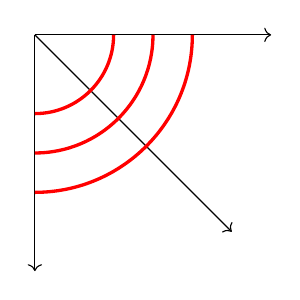
\begin{tikzpicture}
    \draw[->] (0,0) -- (3,0);
    \draw[->] (0,0) -- (2.5,-2.5);
    \draw[->] (0,0) -- (0,-3);
    \draw[red,very thick] (1,0) arc (0:-90:1);
    \draw[red,very thick] (1.5,0) arc (0:-90:1.5);
    \draw[red,very thick] (2,0) arc (0:-90:2);
  \end{tikzpicture}
\end{center}
The direction of the arrows determine the direction of propagation.

\subsubsection*{Reflection}
\begin{center}
  \begin{tikzpicture}
    \draw (-2,0) -- (2,0);
    \draw[dashed] (0,2) -- (0,-2);
    \draw[->] (-2,1) -- (0,0) node[pos=0,above] {object};
    \draw[->] (0,0) -- (2,1);
    \node[above] at (-0.5,0.5) {\( \theta_i \)};
    \node[above] at (0.5,0.5) {\( \theta_f \)};
  \end{tikzpicture}
\end{center}
\[ \theta_i = \theta_f \]
You always see objects as if your line of sight never deviated.

\subsubsection*{Refraction}
\begin{center}
  \begin{tikzpicture}
    \draw (-2,0) -- (2,0);
    \draw[dashed] (0,2) -- (0,-2);
    \draw[->] (-2,1) -- (0,0) node[pos=0,above] {object};
    \draw[->] (0,0) -- (1,-2);
    \node[above] at (-0.5,0.5) {\( \theta_1 \)};
    \node[above] at (0.25,-1.5) {\( \theta_2 \)};
    \node[above] at (-3,0) {air: \( n_1 = 1 \)};
    \node[below] at (-3,0) {water: \( n_2 = 1.3 \)};
  \end{tikzpicture}
\end{center}
Snell's Law:
\[ n_1\sin(\theta_1) = n_2\sin(\theta_2) \]

\subsection*{Interference}
Interference is the interaction of multiple waves.
\begin{center}
  \begin{tikzpicture}[scale=0.4]
    \draw[<->] (0,-2) -- (0,2);
    \draw[->] (0,0) -- (7,0) node[right] {\( x \)};
    \draw (0,0) sin (1,1) cos (2,0) sin (3,-1) cos (4,0) sin (5,1) cos (6,0);
    \node at (9,0) {\( + \)};
  \end{tikzpicture}
  \begin{tikzpicture}[scale=0.4]
    \draw[<->] (0,-2) -- (0,2);
    \draw[->] (0,0) -- (7,0) node[right] {\( x \)};
    \draw (0,0) sin (1,1) cos (2,0) sin (3,-1) cos (4,0) sin (5,1) cos (6,0);
    \node at (9,0) {\( = \)};
  \end{tikzpicture}
  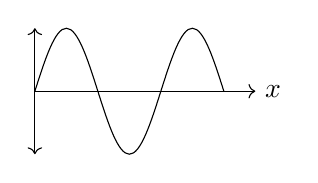
\begin{tikzpicture}[scale=0.4]
    \draw[<->] (0,-2) -- (0,2);
    \draw[->] (0,0) -- (7,0) node[right] {\( x \)};
    \draw (0,0) sin (1,2) cos (2,0) sin (3,-2) cos (4,0) sin (5,2) cos (6,0);
  \end{tikzpicture}
\end{center}
Interference works if the two waves have the same \( \lambda \) and have a
constant phase relationship. For constructive interference:
\[ \Delta r = r_A-r_B = m\lambda \]
For destructive interference:
\[ \Delta r = r_A-r_B = (m+\frac{1}{2})\lambda \]
With light, it is hard to get two coherent sources. Instead, we use a single
light source and split it up using a thin film or partially reflective mirror.

\subsection*{Polarization}
Polarization is the axis on which a wave oscillates.
\begin{center}
  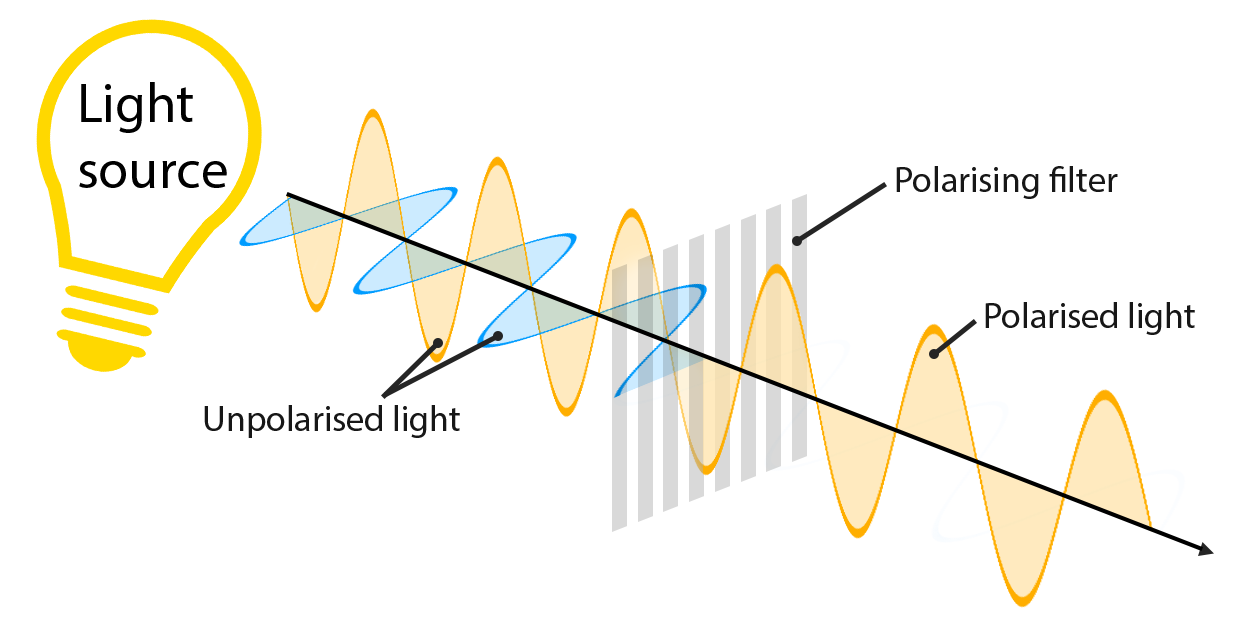
\includegraphics[width=16cm]{assets/polarization.png}
\end{center}
We define the polarization of light as the polarization of light as the
polarization of the electric field, without regard to the perpendicular magnetic
field. Polarizers only let through light which is oriented according to the
polarizer's angle of polarization. Polarized light will have an intensity
relative to the unpolarized light according to the following equation:
\[ I = \frac{I_{\circ}}{2} \]
When you have polarized light passing through a polarized filter:
\[ I = I_{\circ}\cos^2(\phi) \]

\begin{center}
  You can find all my notes at \url{http://omgimanerd.tech/notes}. If you have
  any questions, comments, or concerns, please contact me at
  alvin@omgimanerd.tech
\end{center}

\end{document}
